\input{src/macros.tex}

\title{Cryptanalyse linéaire}
\author{
    William \textsc{Aufort}\\
    Marc \textsc{Chevalier}
}
\date{\today}

\begin{document}
\maketitle

\section*{Question 2}

Notre programme nous donne la matrice $L$ suivante :

\setcounter{MaxMatrixCols}{16}
\[ L = \quad \begin{pmatrix}
16 & 8 & 8 & 8 & 8 & 8 & 8 & 8 & 8 & 8 & 8 & 8 & 8 & 8 & 8 & 8 \\
8 & 10 & 8 & 6 & 8 & 14 & 8 & 10 & 10 & 8 & 6 & 8 & 6 & 8 & 10 & 8 \\
8 & 4 & 8 & 8 & 6 & 10 & 6 & 6 & 8 & 8 & 4 & 8 & 10 & 10 & 6 & 10 \\
8 & 6 & 8 & 6 & 6 & 8 & 6 & 8 & 10 & 8 & 10 & 8 & 8 & 10 & 8 & 2 \\
8 & 10 & 8 & 10 & 8 & 6 & 8 & 6 & 14 & 8 & 6 & 8 & 10 & 8 & 10 & 8 \\
8 & 8 & 4 & 8 & 8 & 8 & 12 & 8 & 8 & 12 & 8 & 8 & 8 & 12 & 8 & 8 \\
8 & 10 & 4 & 10 & 10 & 8 & 6 & 8 & 6 & 4 & 6 & 8 & 8 & 10 & 8 & 6 \\
8 & 8 & 8 & 8 & 10 & 10 & 10 & 2 & 8 & 8 & 8 & 8 & 6 & 6 & 6 & 6 \\
8 & 4 & 6 & 6 & 10 & 6 & 8 & 8 & 8 & 8 & 6 & 10 & 6 & 6 & 12 & 8 \\
8 & 10 & 6 & 8 & 2 & 8 & 8 & 6 & 6 & 8 & 8 & 10 & 8 & 6 & 10 & 8 \\
8 & 8 & 10 & 10 & 8 & 8 & 10 & 10 & 8 & 8 & 6 & 14 & 8 & 8 & 6 & 6 \\
8 & 6 & 10 & 12 & 8 & 10 & 10 & 8 & 6 & 8 & 8 & 6 & 10 & 8 & 12 & 6 \\
8 & 6 & 6 & 8 & 6 & 8 & 12 & 10 & 10 & 4 & 8 & 6 & 8 & 6 & 6 & 8 \\
8 & 8 & 10 & 10 & 6 & 6 & 8 & 8 & 8 & 8 & 6 & 6 & 2 & 10 & 8 & 8 \\
8 & 6 & 6 & 12 & 8 & 10 & 6 & 8 & 10 & 8 & 12 & 10 & 6 & 8 & 8 & 10 \\
8 & 8 & 10 & 6 & 8 & 8 & 10 & 6 & 8 & 4 & 10 & 10 & 8 & 12 & 10 & 10

\end{pmatrix}\]

\section*{Question 3}

Les probabilités les plus éloignées de 0.5 (hormis 1, valeur atteinte pour le couple $(0,0)$) sont 0.125 et 0.875.
Elles sont atteintes respectivement pour les couples :
\begin{enumerate}
\item $p_{3,15} = p_{7,7} = p_{9,4} = p_{13,12} = 0.125$
\item $p_{1,5} = p_{4,8} = p_{10,11} = 0.875$
\end{enumerate}

En effet, il n'est pas très intéressant de travailler avec le couple $(0,0)$ : dans ce cas $a.x = b.S(x) \Leftrightarrow 0 = 0$, qui est une relation dont on ne peut rien déduire...

\section*{Question 4}

\underline{Remarque :} Comme la fin de la question le laisse suggérer, on suppose que les probabilités portent sur le message $m$, et que les clés $K_0$, $K_1$ et $K_2$ sont fixées.

Soit $m$ un message aléatoire distribué (en tant que variable aléatoire) uniformément sur %TODO

Avec les notations introduites dans l'énoncé, on a \[A.m = a.m^{(0)}\] et \[P(B).x_1 = P(B).F(x_0,K_1) = P(B).\left( P \left( S(x_0) \right) \oplus K_1 \right)\]

Soit $K_3$ telle que $K_1 = P(K_3)$. On a :


\[
    \begin{aligned}
        P(B).x_1 &= P(B).\left (P\left (S\left (x_0\right )\right )\oplus P(K_3)\right ) \\
        &= P\left (B\right ).P\left (S\left (x_0\right ) \oplus K_3\right )\\
        &= B.\left (S\left (x_0\right ) \oplus K_3\right ) \\
        &= b.\left (S\left (x_0^{\left (0\right )}\right ) \oplus K_3^{(0)}\right )
    \end{aligned}
\]

D'où $\prob{A.m = P(B).x_1} = \prob{a.m^{(0)}= b.(S(x_0^{(0)}) \oplus K_3^{(0)})}$.

Avec $x_0^{(0)} = m^{(0)} \oplus K_0^{(0)}$.

Pour se ramener aux probabilités introduites dans la matrice $L$ (i.e du type $\prob{a.y = b.S(y)}$), l'idée est d'observer que l'utilisation des clés ne changent pas la distribution uniforme.

\begin{lemma}
	Si $x$ est uniforme, alors $x \oplus K$ est uniforme pour tout clé $K$.
\end{lemma}

\begin{proof}
	Il suffit de montrer que chaque bit de $x \oplus K$ est uniformément distribué dans $\{0,1\}$.

	Soit $x_i$ un bit aléatoire de $x$. Le ième bit de $x \oplus K$ est $x_i \oplus K_i$.

	Si $K_i = 0$, $x_i \oplus K_i = x_i$ donc uniforme.

	Si $K_i = 1$, $x_i \oplus K_i = 1 - x_i$ également uniforme. 
\end{proof}

\begin{lemma}
	Si $x$ est uniforme, alors $S(x)$ et $P(x)$ aussi.
\end{lemma}
\begin{proof}
	Clair car $S$ et $P$ sont des bijections.
\end{proof}

Avec ces deux lemmes, on peut maintenant écrire :

\begin{align*}
\prob{a.m^{(0)}= b.\left (S\left (x_0^{(0)}\right ) \oplus K_3^{(0)}\right )} &= \prob{a.m^{(0)} = b.(S(x_0^{(0)}))} \\
													&= \prob{a.\left(x^{(0)} \oplus K_0^{(0)}\right ) =  b.\left (S\left (x_0^{(0)}\right )\right )} \\
													&= \prob{a.x^{(0)} = b.\left(S\left(x_0^{\left(0\right)}\right)\right)} \\
													&= \frac{1}{2} \pm \frac{6}{16}
\end{align*}
Car $0.125 = \frac{1}{2} - \frac{6}{16}$ et $0.875 = \frac{1}{2} + \frac{6}{16}$.

D'où $\prob{A.m = P(B).x_1} = \frac{1}{2} \pm \frac{6}{16}$, ce qui permet de conclure.

\section*{Question 5}

Selon la valeur de $b$, les bits non nuls de $P(B)$ peuvent correspondre à une ou deux Sboxes (le "ou" ayant un sens exclusif ici). C'est ce qu'on entend par les cas "une boîte active" et "deux boîtes actives" (notamment dans la question 8).

En effet, avec les $A$ et $B$ donnés, les seuls bits de $K_2$ qui vont intervenir dans le calcul de $P(B).x1$ sont les bits $i$ tels que $P(B)_i \neq 0$. Ces bits font forcément partis des bits de $b$, qui sont situés entre les rangs 2 et 6 (voir figure 
\ref{illustration_bits_key}).

Si les bits de $b$ valant $1$ occupent deux groupes de 4 bits différents (qui correspondent aux résultats de 2 boxes différentes), on est dans le cas "deux actives boxes". C'est le cas de la figure \ref{illustration_bits_key}. Dans ce cas, on peut se limiter à chercher les 8 premiers bits de la clé.


\begin{figure}[!ht]
\centering
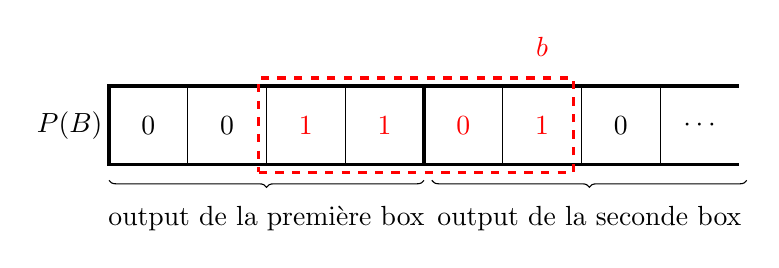
\begin{tikzpicture}
	\draw[very thick] (8,1) -- (0,1) -- (0,0) -- (8,0) ;
	\draw[very thick] (4,0) -- (4,1);
	\draw[decorate,decoration={brace,raise=0.2cm}] (4,0) -- (0,0) node[below=0.4cm,pos=0.5] {output de la première box};
	\draw[decorate,decoration={brace,raise=0.2cm}] (8.1,0) -- (4.1,0) node[below=0.4cm,pos=0.5] {output de la seconde box};
	\draw (1,0) -- (1,1);
	\draw (2,0) -- (2,1);
	\draw (3,0) -- (3,1);
	\draw (5,0) -- (5,1);
	\draw (6,0) -- (6,1);
	\draw (7,0) -- (7,1);
	\draw[very thin] (0.5,0.5) node {$0$};
	\draw[very thin] (1.5,0.5) node {$0$};
	\draw[very thin,color=red] (2.5,0.5) node {$1$};
	\draw[very thin,color=red] (3.5,0.5) node {$1$};
	\draw[very thin,color=red] (4.5,0.5) node {$0$};
	\draw[very thin,color=red] (5.5,0.5) node {$1$};
	\draw[very thin] (6.5,0.5) node {$0$};
	\draw[very thin] (7.5,0.5) node {$\cdots$};
	\draw[dashed, very thick, color=red] (1.9,-0.1) -- (5.9,-0.1) -- (5.9,1.1) -- (1.9,1.1) -- cycle;
	\draw[color=red] (5.5,1.5) node {$b$};
	\draw (-0.5,0.5) node {$P(B)$};
\end{tikzpicture}
\caption{Ici on cherche à deviner 8 bits de $K_2$ (cas où l'on deux boîtes actives)}
\label{illustration_bits_key}
\end{figure}


S'ils occupent un seul groupe, alors on est dans le cas "une boîte active". On peut alors se limiter à deviner les 4 premiers bits (ou les 4 suivants selon $b$) de la clé $K_2$.

Il est facile de voir que l'on est dans le cas "une boîte active" si $b < 3$ (seuls les bits à droite sont non nuls), ou si $4$ divise $b$ (seuls les bits à gauche sont non nuls).

L'algorithme qui renvoie les 4 bits les plus probables pour la sous-clé qui nous intéresse est donné ci-dessous. Dans cet algorithme, nous ne devinons que 4 bits pour les deux méthodes. Nous expliquerons ce choix à la question 8.

\begin{algorithm}
\caption{L'attaque des 4 bits de la clé pouvant être devinés}
	\Entree{Des couples $(m,c)$}
	\Sortie{La sous-clé $K'_2$ la plus probable}
	$n \longleftarrow $ nombre de couples plaintexts/ciphertexts à disposition. \\
	\Pour{chaque couple $(a,b)$ du bon type (une ou deux boîtes actives)}
	{
		\Pour{chaque clé $K'_2 \in \{0,1\}^4$}
		{
			\Pour{Chaque couple $(m,c)$}
			{
				Calculer $x_1 = c \oplus K_2$ ($K_2$ = $K'_2$ complétée par des zéros ailleurs) \\
				\Si{$A.m = P(B).x_1$}{$Count[K'_2]$++}
			}
		$Biais[K'_2] = | Count[K'_2] - n |$
		}
		
	}
	\Retour{$Argmin \left( Biais[.] \right)$}
\end{algorithm}

\section*{Question 6}

Dans toute cette table, les bits de $m$ seront notés m = $m_0 m_1\cdots m_n$, et les bits de $x_1$ (que l'on renomme $x$) seront notés $x_1 = x_0 x_1 \cdots x_n$. On fera notamment attention au fait que, dans ce tableau, $x_1$ désignera le deuxième bit de $x$ fraîchement renommé.

Par mesure de simplicité, on ne représente qu'une partie des bits nuls de P(B).

\begin{table}[!ht]
\centering
\begin{small}
\begin{tabular}{|c|c|c|c|c|c|}
	\hline
	$(a,b)$   & $p_{a,b}$ & 		$P(B)$ 	   & équation linéaire	 & \# de boîtes actives & bits de $K_2$ à deviner \\
	\hline
	$(3,15)$  &   0.125   & $0011110\cdots0$ & $m_2 \oplus m_3 = x_0 \oplus x_1 \oplus x_2 \oplus x_3$ & 2 & 2, 3, 4, 5 \\
	\hline
	$(7,7)$   &   0.125   & $0001110\cdots0$ & $m_1 \oplus m_2 \oplus m_3 = x_1 \oplus x_2 \oplus x_3$ & 2 & 3, 4, 5\\
	\hline
	$(9,4)$   &   0.125   & $0001000\cdots0$ & $m_0 \oplus m_3 = x_1$ 								   & 1 & 3 \\
	\hline
	$(13,12)$ &   0.125   & $0011000\cdots0$ & $m_0 \oplus m_1 \oplus m_3 = x_0 \oplus x_1$ 		   & 1 & 2, 3 \\
	\hline
	$(1,5)$   &   0.875   & $0001010\cdots0$ & $m_3 = m_1 \oplus m_3$								   & 2 & 3, 5 \\
	\hline
	$(4,8)$   &   0.875   & $0010000\cdots0$ & $m_1 = x_0$ 											   & 1 & 2 \\
	\hline
	$(10,11)$ &   0.875   & $0010110\cdots0$ & $m_0 \oplus m_2 = x_0 \oplus x_2 \oplus x_3$			   & 2 & 2, 4, 5 \\
	\hline
\end{tabular}
\end{small}
\caption{Le tableau global regroupant tous les éléments nécessaires à l'attaque}
\end{table}

\section*{Question 7}

%TODO : Trouver le pari spécifique à un couple (a,b)

\section*{Question 8}

\subsection*{Efficacité des deux méthodes}

Plusieurs méthodes ont été testées : couple par couple, moyenne des couples (une ou deux boîtes actives). Tout d'abord, les différents couples ne donnent pas en soi les mêmes clés $K_2$, et sachant que l'on a peu de couples $(a,b)$, on ne pouvait pas choisir lequel des paquet de 4 bits prendre à chaque passe. Nous avons donc implémenté une méthode qui choisit la bonne clé en regardant la somme des biais (écart à la valeur moyenne). Cette méthode fonctionne très bien avec deux boîtes actives, par contre on observe quelques erreurs avec une seule boîte active pour certains choix de couples, alors que pour d'autres le résultat est identique. En effet, avec les couples données, par exemple seuls les bits 2 et 3 peuvent être facilement déduits d'après le tableau (ce qui n'est pas le cas des bits 4 et 5). Ceci est du au fait que tous les $b$ sont dans une seule des deux catégories énoncées en question 5 (en l'occurrence, $b$ multiple de $4$).

\subsection*{Complexité}

%TODO : Ici, il faudra comparer les deux méthodes par rapport à la vitesse d'exécution et au nombre d'opérations effectuées

Pour comparer la complexité des deux méthodes, il suffit de comparer la complexité de la recherche de la première clé $K_2$. En effet, après avoir trouvé $K_2$, on n'utilise plus du tout les boîtes actives.

Dans l'algorithme que nous avons implémenté, le fait d'utiliser une ou deux boîtes actives donne exactement la même complexité. En effet, à chaque fois, on cherche à deviner le même nombre de bits, et les calculs à effectuer sont les mêmes.

On va chercher à comparer ici un algorithme différent : avec deux boîtes actives, on pourrait chercher à deviner la clé par bloc de 8 (les 8 bits appartenant aux deux boîtes), alors qu'avec une boîte active, on pourrait chercher à deviner la clé par bloc de 4, mais face aux boîtes (et non pas en décalé comme cela a été implémenté).

Soit $C(n)$ le coût d'un produit scalaire entre deux nombres de $n$ bits. On peut supposer que $C(n)$ est linéaire.

Le coût de chaque méthode est donné par $ \# (subkeys) \times 2^{ | keys |} \times 2 C( |keys|)$. En effet, il faut deviner $\# (subkeys)$ sous-clés, avec une méthode qui nécessite de tester $2^{ | keys |}$ sous-clés possibles, ces tests utilisant essentiellement deux calculs de produits scalaires.

Pour la méthode avec une boîte active, ce coût vaut $C_1 = 8 \times 2^4 \times 2 C(8)$. 

Pour la méthode avec deux boîtes actives, ce coût vaut $C_2 = 4 \times 2^8 \times 2 C(4)$.

La gain entre ces deux méthodes vaut alors :

$$ \frac{C_2}{C_1} = \frac{1}{2} \times 2^{8-4} \times \frac{C(8)}{C(4)} = 16$$.

La méthode utilisant une boîte active va donc 16 fois plus vite que l'autre méthode.

En pratique, nous avons utilisé des deux boîtes actives, mais avec un algorithme qui ne devine que des blocs de 4 bits correspondant précisément aux bits sur lesquels les relations intervenants dans la table de la question 6 opèrent.

\section*{Question 9}

Une fois que l'on a trouvé la clé $K_2$, on peut se ramener à l'étude d'un schéma de chiffrement utilisant seulement un tour de fonction $F$. Pour cela, il suffit, à partir de la clé trouvée et du fonctionnement des boîtes, de retrouver $x_1 = F(x_0,K_1) = F^{-1}(c,K_2)$.

On a alors, dans ce schéma de chiffrement réduit, un jeu de couple $(m,x_1)$ où les $x_1$ correspondent au résultat du chiffrement de chaque $m$.

Pour trouver les clés $K_0$ et $K_1$, on ne peut plus utiliser la relation précédente. Il faut se débrouiller autrement. L'idée ici est de deviner $K_0$ par bloc. On remarque qu'à partir d'un bloc de $K_0$, pour chaque couple $(m,x_1)$, on peut construire un bloc $K_1 = F(m \oplus K_0) \oplus x_1$, la seule clé qui puisse convenir. Ensuite, on compte pour chaque pari le nombre de couples tels que les relations que doivent vérifier les bits de $K_0$ et $K_1$ et ceux déjà découverts de $K_2$. Enfin, on ne garde que les sous-clés tel que le nombre de couples est maximal (égal précisément au nombre de couples).	

Finalement, à partir des trois clés $K_2$, $K_1$ et $K_0$, il est facile de retrouver la clé $K$ à partir de la table des permutations utilisées pour construire les trois clés. De plus, on peut vérifier pendant cette étape que l'on a effectivement bien trouver les bonnes clés lors des étapes précédentes.

\end{document}

